\chapter[Metodologia]{Metodologia}
\section{Proposta Geral}

A evolução dos equipamentos de mixagem começou com a mixagem em vinil, e ao longo do tempo, novas funcionalidades foram adicionadas, como o \textit{jogger} para atraso e avanço da música, \textit{fader} para controle de volume e \textit{knobs} para ajuste de frequências. Com o avanço da microeletrônica, esses equipamentos evoluíram para a eletrônica digital, incorporando \textit{DSPs} para processar formatos de áudio de alta qualidade, como WAV e FLAC.

Atualmente, existem dois tipos principais de equipamentos de mixagem: os mais caros, que não requerem um computador, e os mais acessíveis, que dependem de um computador, mas oferecem melhor qualidade de processamento. DJs iniciantes frequentemente enfrentam dificuldades para realizar ajustes finos nas bandas de frequência em \textit{mixers} clássicos de três bandas. Esta habilidade é crucial para destacar elementos musicais e criar novas atmosferas. À medida que um DJ desenvolve seu estilo, a mixagem torna-se mais automática, facilitando a transição entre músicas.

Este projeto propõe a criação de um \textit{mixer} com um controle central que manipula dois canais de entrada (duas músicas). Em vez dos tradicionais controles de três bandas de frequência, o mixer utilizará filtros passa-altas. O controle central ajustará simultaneamente as frequências de corte de ambos os canais, permitindo uma transição suave entre as músicas.

Além disso, o sistema incluirá dois efeitos, \textit{delay} e \textit{reverb}, que serão controlados automaticamente pela posição do botão central. Quando o botão estiver na posição intermediária, os efeitos serão aplicados ao máximo, diminuindo gradualmente conforme o botão se move para uma das extremidades.

Em resumo, o sistema processará sinais de áudio analógicos em tempo real, utilizando filtros passa-altas e permitindo ao usuário selecionar e controlar a intensidade dos efeitos, com botões \textit{sliders} para ajuste e um botão \textit{on}/\textit{off} para seleção dos efeitos.

\section{Levantamento de Requisitos}

O levantamento de requisitos é uma etapa crucial no desenvolvimento de qualquer sistema, pois define as funcionalidades e características necessárias para atender às necessidades dos usuários finais. Nesta seção, são apresentados os requisitos funcionais e não funcionais, que especificam o comportamento esperado do sistema, assim como as restrições e qualidades que devem ser atendidas. Os requisitos foram organizados em categorias que abrangem desde aspectos de desempenho e interface do usuário até segurança e manutenção, assegurando uma visão completa e detalhada do que o sistema deve entregar.

\subsection{Requisitos Funcionais}
\begin{itemize}
    \item O sistema deve permitir ao \textit{DJ} utilizar tanto \textit{CDJs} quanto toca-discos.
    \item O sistema deve permitir ao \textit{DJ} controlar a presença dos dois \textit{canais}.
    \item O sistema deve permitir ao \textit{DJ} controlar a presença dos efeitos.
\end{itemize}

\subsection{Requisitos Não-Funcionais}
\begin{itemize}
    \item O sistema deve responder aos comandos do \textit{DJ} com latência mínima, garantindo uma experiência de mixagem fluida.
    \item A interface do usuário deve ser intuitiva e fácil de usar, permitindo que o \textit{DJ} faça ajustes rapidamente durante a performance.
    \item O sistema deve ser confiável e estável, capaz de lidar com longos períodos de uso contínuo sem falhas.
    \item O sistema deve oferecer uma qualidade de som de alta fidelidade, garantindo que o áudio reproduzido seja claro e com mínimas distorções.
    \item A interface do mixer deve incluir botões físicos ou controles táteis para ajuste de frequência e efeitos de áudio.
    \item A interface do mixer deve ser organizada de forma lógica e intuitiva, com controles agrupados por função para facilitar a navegação.
    \item A interface deve possuir indicações claras das funções dos botões de interação com o usuário.
    \item O sistema deve ser compatível com uma variedade de dispositivos de áudio externos, como \textit{CDJs} e toca-discos.
    \item O sistema deve ser alimentado por uma fonte de energia padrão, como uma tomada elétrica.
    \item O sistema deve incluir interfaces de entrada e saída de áudio padrão \textit{RCA}.
    \item O sistema deve ser capaz de lidar com até dois \textit{canais} de áudio simultaneamente, sem comprometer a qualidade do som ou a responsividade dos controles.
    \item O sistema deve suportar uma ampla gama de frequências de áudio, garantindo que os graves sejam reproduzidos com profundidade e os agudos sejam nítidos e claros.
    \item O sistema deve ser projetado para minimizar o risco de danos aos equipamentos de áudio conectados, oferecendo proteção contra sobrecarga ou curto-circuito.
    \item O sistema deve ser projetado para facilitar a manutenção e reparo, com acesso fácil aos componentes internos e documentação clara sobre procedimentos de serviço.
    \item O sistema deve ser capaz de se comunicar perfeitamente com qualquer dispositivo de reprodução de música profissional, tanto como canal de entrada quanto como sistema de som de saída.
\end{itemize}



\section{Fluxograma do Mixer}

O \textit{mixer} proposto é composto por subblocos de funcionamento interligados, conforme ilustrado na Figura \ref{fig52}.

De forma geral, o sistema opera em um ciclo contínuo de leitura de sinais, tanto das músicas quanto dos controles, e realiza modificações de parâmetros para processar os sinais, que, por fim, são reproduzidos. Cada ciclo pode ser representado na Figura \ref{fig52}.

\begin{figure}[h]
    \centering
    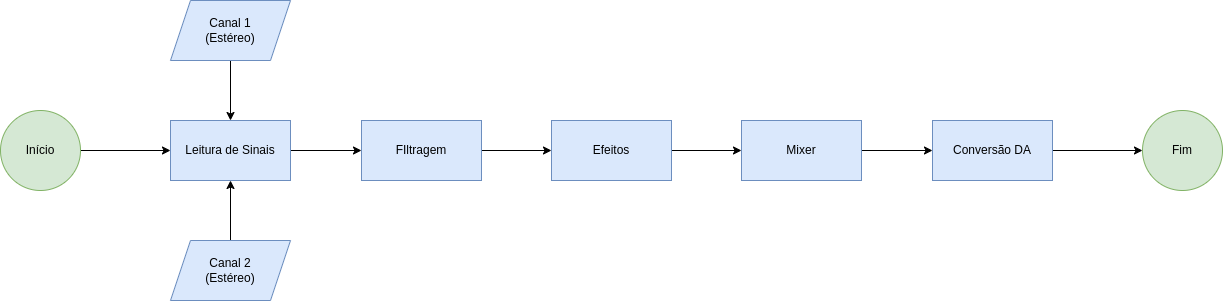
\includegraphics[width=\textwidth]{figuras/fig52.png}
    \caption{fluxograma geral do \textit{mixer}}
    \label{fig52}
\end{figure}

Os sinais provenientes dos dispositivos de reprodução de música entram no sistema e são convertidos para sinais digitais. Simultaneamente, é feita uma leitura dos valores atuais dos controles disponíveis na interface.

Com os valores dos parâmetros obtidos, a filtragem dos sinais e o processamento dos efeitos são realizados novamente para ajustar o comportamento dos sinais conforme os novos valores dos controles.

Finalmente, os sinais filtrados e os efeitos são combinados e convertidos para o formato analógico, para que possam ser reproduzidos.

Nas subseções abaixo, cada bloco presente no fluxograma geral do sistema (Figura \ref{fig52}) será detalhado em seus aspectos conceituais e processuais por meio de um subfluxograma, que descreve o processamento interno.

\subsection{Bloco de Leitura de Sinais}

Os sinais analógicos lidos incluem os sinais de música e os sinais de controle provenientes de dois potenciômetros e um botão de duas posições. Os potenciômetros são utilizados para ajustar a frequência central e a quantidade de efeito desejado, enquanto o botão de duas posições é utilizado para selecionar o efeito desejado.

\begin{figure}[h]
    \centering
    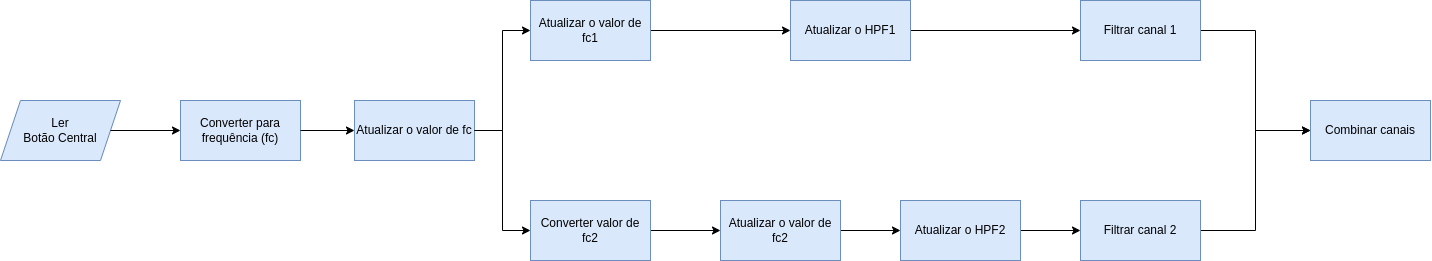
\includegraphics[width=\textwidth]{figuras/fig54.png}
    \caption{bloco de leitura de sinais analógicos}
    \label{fig54}
\end{figure}

As operações realizadas nesses sinais são ilustradas na Figura \ref{fig54}.

\subsection{Bloco de Filtragem}

No bloco de filtragem, os sinais já estão no domínio digital. Primeiramente, deve-se ler a posição do botão central, que é obtida a partir da conversão de um sinal analógico proveniente de um potenciômetro, convertido de um sinal elétrico para um sinal digital.

Com a posição do botão, que estará em um intervalo de valores quantizados, realiza-se a normalização e conversão para um valor de frequência de corte, variando entre 20 e 22.050 Hz.

Este valor de frequência de corte é utilizado para atualizar o filtro passa-altas do canal 1, que então realiza a filtragem do sinal correspondente.

Para o canal 2, um novo valor de frequência de corte é calculado usando a expressão da Equação \ref{eq:05}. O filtro passa-altas deste canal é então ajustado conforme a nova frequência de corte, conforme ilustrado na Figura \ref{fig55}.

No bloco de filtragem, todos os sinais analógicos já estão codificados de forma que podem ser processados digitalmente. A frequência de corte central (\textit{fc}) varia entre 20 e 22.050 Hz, e os valores são atribuídos aos parâmetros \textit{fc$_{1}$} e \textit{fc$_{2}$}.

\begin{figure}[h]
    \centering
    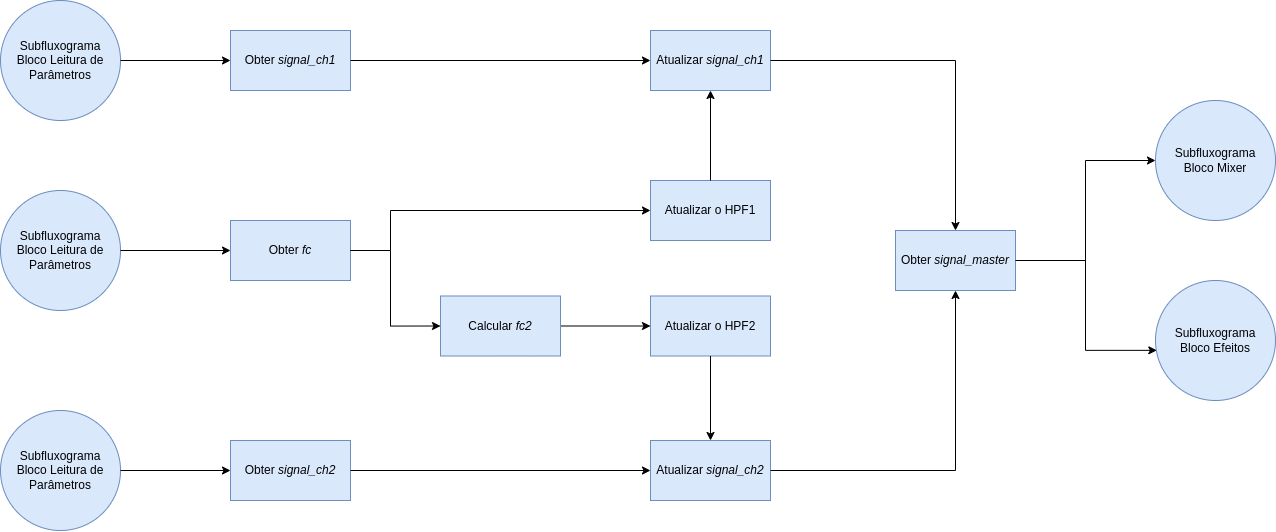
\includegraphics[width=\textwidth]{figuras/fig55.png}
    \caption{bloco de filtragem}
    \label{fig55}
\end{figure}

No subfluxograma da Figura \ref{fig55}, \textit{fc} representa a frequência de corte central, lida e convertida a partir do botão central; \textit{fc$_{1}$} é a frequência de corte para o filtro passa-altas 1 (HPF1) e \textit{fc$_{2}$} é a frequência de corte para o filtro passa-altas 2 (HPF2).

Ao final deste processo, os sinais dos dois canais são combinados, resultando no sinal \textit{signal\_master}, que é enviado tanto para o bloco de processamento de efeitos quanto para o bloco final de combinação dos sinais: o sinal de efeito e a combinação dos canais 1 e 2.

\subsection{Bloco de Efeitos}

Os efeitos do \textit{mixer} podem ter seus parâmetros de reverberação e atraso configurados conforme o botão de quantidade de efeito. O parâmetro de reverberação é ajustado para 1 segundo, e o intervalo de atraso (em milissegundos) é configurado de acordo com a quantidade de efeito desejado.

\begin{figure}[h]
    \centering
    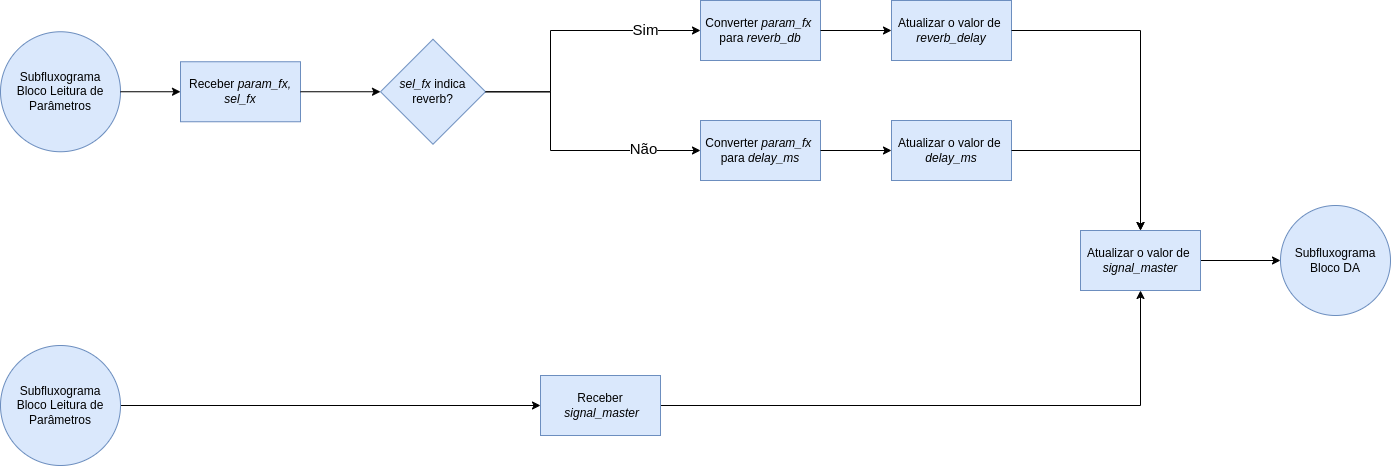
\includegraphics[width=\textwidth]{figuras/fig56.png}
    \caption{bloco de efeitos}
    \label{fig56}
\end{figure}

Além disso, o usuário pode selecionar qual efeito deseja utilizar através de um botão de duas posições, conforme ilustrado na Figura \ref{fig56}. Os parâmetros de seleção e quantidade de efeitos são obtidos do bloco de leitura de sinais. Ao final deste bloco, o sinal isolado do efeito, com o efeito aplicado, é atribuído ao \textit{signal\_fx}.

\subsection{Bloco de Automação de Efeitos}

No \textit{mixer} proposto, o volume do efeito é ajustado automaticamente conforme a frequência central, como ilustrado na Figura \ref{fig57}. Quando a frequência de corte central (\textit{fc}) está nas extremidades do intervalo, o volume do efeito é nulo. À medida que a \textit{fc} se aproxima da posição central da banda de frequência, o volume do efeito aumenta gradualmente.

\begin{figure}[h]
    \centering
    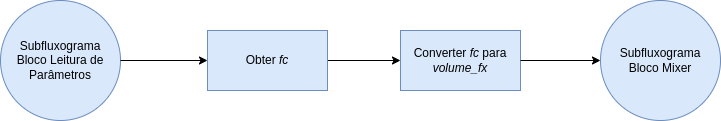
\includegraphics[width=\textwidth]{figuras/fig57.png}
    \caption{bloco de automação do volume de efeitos}
    \label{fig57}
\end{figure}

Para calcular o ganho do efeito, uma expressão é utilizada para converter o valor da \textit{fc} em \textit{volume\_fx}, que representa o ganho do \textit{signal\_fx}.

\subsection{Bloco Mixer}

O processo de mistura de dois sinais é conhecido como \textit{mixing}. Neste \textit{mixer}, há dois momentos distintos em que os sinais são misturados: primeiro, os sinais dos canais 1 e 2 são combinados; depois, os sinais já combinados dos canais 1 e 2 são misturados com o sinal do efeito. Este bloco refere-se à mistura final, ou seja, a segunda etapa do processo.

\begin{figure}[h]
    \centering
    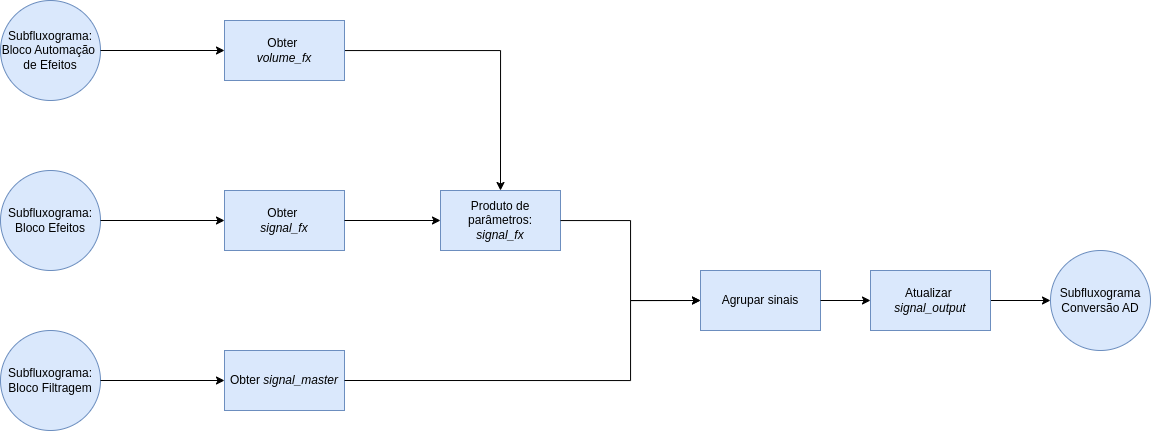
\includegraphics[width=\textwidth]{figuras/fig58.png}
    \caption{bloco de mistura final de sinais}
    \label{fig58}
\end{figure}

No subfluxograma da Figura \ref{fig58}, o sinal do efeito é ajustado em termos de atenuação ou amplificação com base no volume calculado pelo bloco de automação de efeitos. Este sinal de efeito, com o volume ajustado, é então misturado com o sinal proveniente do bloco de filtragem, resultando no sinal de saída, \textit{signal\_output}. No entanto, este sinal ainda está no domínio digital.

\subsection{Bloco de Conversão DA}

O sinal de saída obtido pelo bloco \textit{mixer} precisa ser convertido de digital para analógico para que possa ser reproduzido em um sistema de som.

\begin{figure}[h]
    \centering
    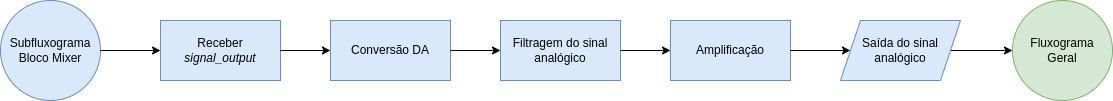
\includegraphics[width=\textwidth]{figuras/fig59.png}
    \caption{bloco de conversão digital-analógico}
    \label{fig59}
\end{figure}

Conforme mostrado na Figura \ref{fig59}, o sinal digital passará por um processo de conversão digital-analógico, seguido por filtragem e amplificação de potência para que possa ser finalmente reproduzido por caixas de som.

\newpage
\section{Prova de Conceito}

Nesta seção, é apresentada uma implementação em um ambiente virtual que simula a lógica de funcionamento do sistema.

\subsection{\textit{PureData}}

O \textit{PureData} \cite{puredata} é um ambiente de música computacional programável, projetado para análise, síntese e processamento de áudio em tempo real através de sinais digitais.

Esse ambiente permite a criação de sistemas de processamento de áudio utilizando blocos programáveis, com funções implementadas tanto pelos seus criadores quanto pela extensa comunidade de usuários. No \textit{PureData}, foi possível desenvolver uma prova de conceito que abrange a lógica do botão central para controle das frequências de corte, bem como o funcionamento dos efeitos. Para simular os sinais de entrada, foram utilizados arquivos WAV locais.

A demonstração do sistema se divide em duas principais funcionalidades: filtragem e efeitos.

\subsection{Implementação de Filtragem}

A filtragem é realizada lendo dois arquivos de música no formato WAV, utilizando as funções \texttt{open}, \texttt{start} e \texttt{stop} para localizar, iniciar e parar a reprodução, respectivamente. Em seguida, o comando \texttt{readsf\textasciitilde\ 2 1e+06} é utilizado para configurar a leitura dos sinais em estéreo com um milhão de amostras no \textit{buffer}. Este processo é repetido para ambos os arquivos.

Para aplicar a filtragem, utiliza-se a função \texttt{hip\textasciitilde}, que implementa um filtro passa-altas. No entanto, o argumento da função varia entre o canal 1 e o canal 2. Como mostrado na Figura \ref{fig24}, o canal 1 ("FC do HPF1") recebe diretamente o parâmetro \textit{fc}, proveniente do \textit{slider} azul.

Por outro lado, o filtro passa-altas do canal 2 ("FC do HPF2") utiliza um valor ajustado por uma expressão anterior, conforme a Equação \ref{eq:05}. Esse ajuste assegura que uma pequena variação em \textit{fc$_{1}$} resulte em uma grande variação em \textit{fc$_{2}$}, e vice-versa. Além disso, em frequências centrais, a variação entre os canais torna-se mais semelhante. A Equação \ref{eq:05} descreve um círculo com raio igual à frequência de amostragem, com o botão centralizado no ponto (22050, 22050).

\begin{equation}  \label{eq:05}
    fc_2 = 22050 - \sqrt{22050^2 - (fc - 22050)^2}
\end{equation}

O ajuste na Equação \ref{eq:05} é projetado para ponderar mudanças nas frequências, pois mudanças lineares não são eficazes com um controle centralizado, como demonstrado pelas frequências dos canais na Figura \ref{fig45}.

\begin{figure}[h]
    \centering
    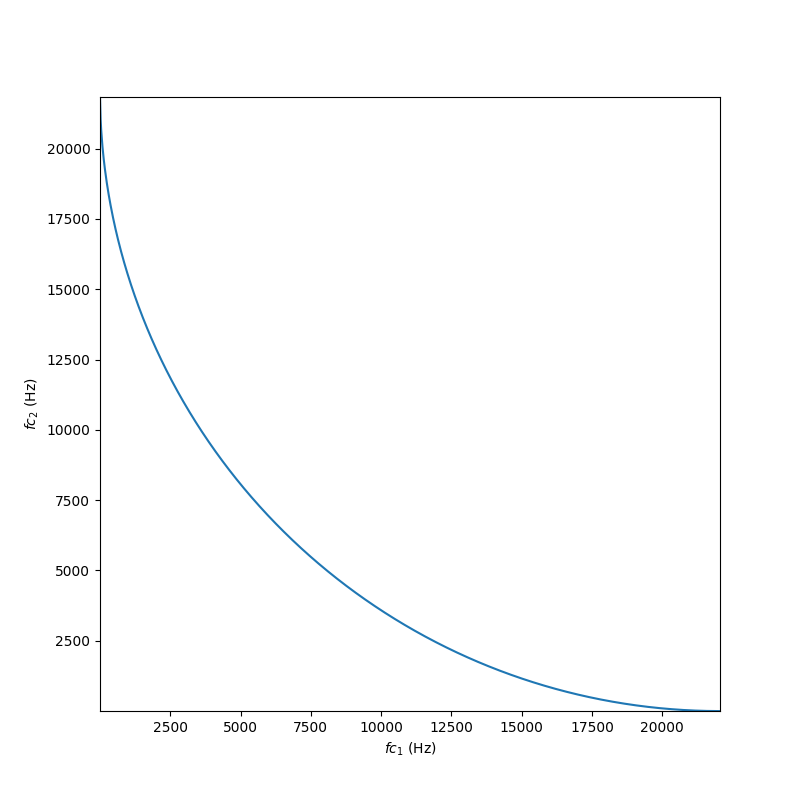
\includegraphics[width=0.7\textwidth]{figuras/fig45.png}
    \caption{expressão para a \textit{fc$_{2}$}}
    \label{fig45}
\end{figure}

Mudanças na ordem de centenas no canal 1 têm pouco impacto no canal 2, uma vez que as baixas frequências têm um ganho maior em relação às altas frequências. Essa lógica também se aplica ao outro extremo do controle de frequência.

\begin{figure}[h]
    \centering
    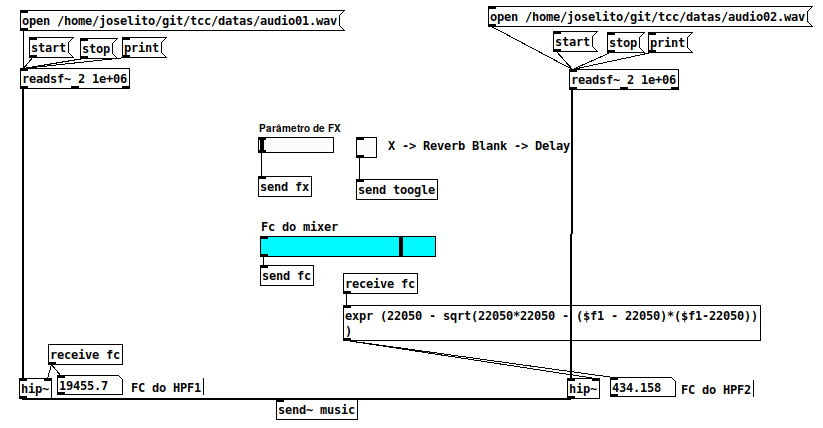
\includegraphics[width=0.9\textwidth]{figuras/fig44.png}
    \caption{lógica de funcionamento do botão central no \textit{PureData}}
    \label{fig44}
\end{figure}

Na Figura \ref{fig44}, a frequência obtida do botão central, denotada como \( f_c \), varia de 0.2 a 22050 Hz. A frequência de corte do canal 1, referida como FC do HPF1, é equivalente a \( f_c \). A frequência de corte do canal 2, identificada como FC do HPF2, é calculada pela Equação \ref{eq:05}. O sinal resultante, \texttt{send\textasciitilde\ music}, é a soma dos sinais filtrados dos canais 1 e 2.

\subsection{Implementação de Efeitos}

A implementação dos efeitos utiliza três parâmetros principais: um botão \texttt{toggle} para alternar entre os efeitos \textit{delay} e \textit{reverb}; um \textit{slider} para ajustar parâmetros internos dos efeitos; e a frequência de corte do botão central, que automatiza o volume do efeito.

O botão \texttt{toggle} é usado para alternar entre os efeitos. Com duas posições disponíveis, sempre um efeito está ativo. Para mudar o efeito, basta alterar a posição do botão, conforme mostrado na Figura \ref{fig46}.

\begin{figure}[h]
    \centering
    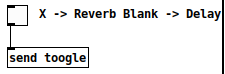
\includegraphics[width=0.3\textwidth]{figuras/fig46.png}
    \caption{botão de seleção de efeito no \textit{PureData}}
    \label{fig46}
\end{figure}

O \textit{slider} é utilizado para ajustar os parâmetros internos de cada efeito. Seus valores variam de 0 a 1, e o botão está ilustrado na Figura \ref{fig47}.

\begin{figure}[h]
    \centering
    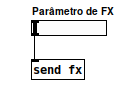
\includegraphics[width=0.2\textwidth]{figuras/fig47.png}
    \caption{botão de quantidade de efeito no \textit{PureData}}
    \label{fig47}
\end{figure}

Cada efeito utiliza o parâmetro \textit{fx} do \textit{slider} e o ajusta conforme necessário. No caso do \textit{reverb}, o valor de \textit{fx} é multiplicado por 100 para determinar a quantidade de \textit{dB} que permanece na música após 1s. Para o \textit{delay}, o valor é multiplicado por 1000, transformando-se no intervalo de tempo em \textit{ms} que o efeito permanecerá na música.

A lógica de seleção do efeito é apresentada na Figura \ref{fig48}. Os comandos \texttt{receive\textasciitilde\ fx} inserem os efeitos como entrada. Cada volume do efeito é multiplicado pelo valor do \texttt{toggle}; um deles é multiplicado pelo valor atual enquanto o outro é multiplicado pelo inverso, permitindo que o botão \texttt{toggle} funcione como um alternador entre os efeitos.

\begin{figure}[h]
    \centering
    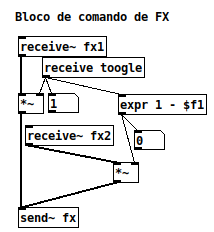
\includegraphics[width=0.3\textwidth]{figuras/fig48.png}
    \caption{lógica de seleção de efeito no \textit{PureData}}
    \label{fig48}
\end{figure}

No sistema, o volume do efeito é ajustado automaticamente com base na posição do botão central, ou seja, nas frequências de corte. A Figura \ref{fig49} ilustra a variação do volume dos efeitos em função da frequência central.

\begin{figure}[h]
    \centering
    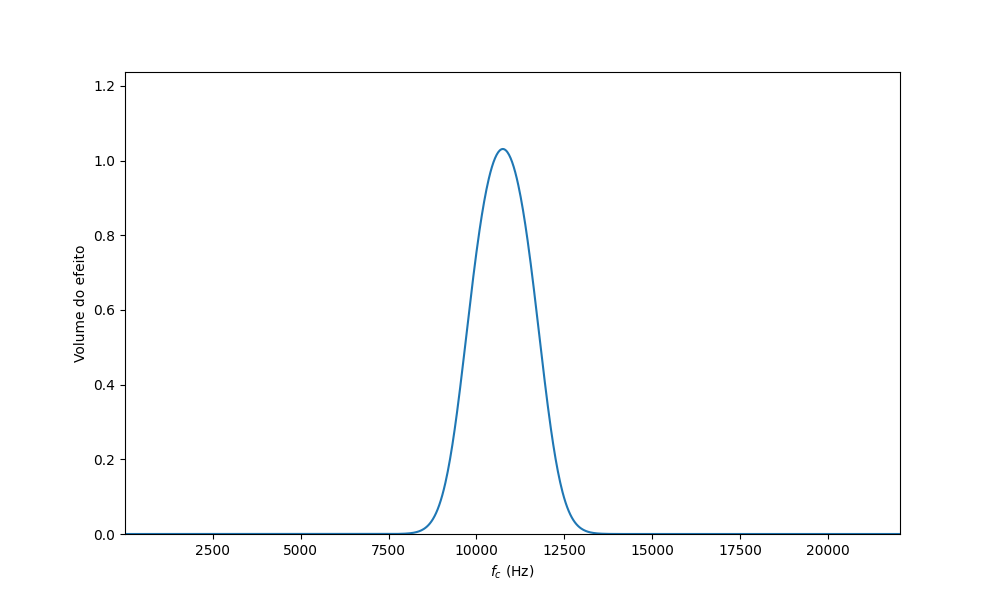
\includegraphics[width=0.9\textwidth]{figuras/fig49.png}
    \caption{variação do volume dos efeitos no \textit{PureData}}
    \label{fig49}
\end{figure}

No \textit{PureData}, o bloco de automação do volume dos efeitos é implementado usando as operações mostradas na Figura \ref{fig50}.

\begin{figure}[h]
    \centering
    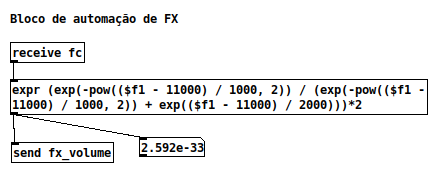
\includegraphics[width=0.6\textwidth]{figuras/fig50.png}
    \caption{implementação da variação do volume dos efeitos no \textit{PureData}}
    \label{fig50}
\end{figure}

Finalmente, o sinal dos efeitos é multiplicado pelo volume dos efeitos e, em seguida, somado ao sinal filtrado, resultando no sinal de saída. Esse sinal é processado por um bloco de conversão digital-analógico e, por fim, é reproduzido. O bloco que realiza a soma dos sinais está representado na Figura \ref{fig51}.

\begin{figure}[h]
    \centering
    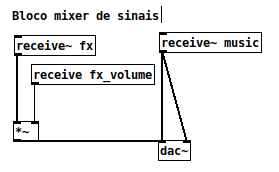
\includegraphics[width=0.3\textwidth]{figuras/fig51.png}
    \caption{soma dos sinais filtrados e dos efeitos no \textit{PureData}}
    \label{fig51}
\end{figure}


\section{Proposta de Implementação}

\subsection{Implementação em Hardware}

Esta seção descreve a proposta de implementação em hardware para o sistema de mixagem de áudio, abrangendo conectores, botões e outros componentes essenciais.

\paragraph{Conectores}
Para a aquisição dos sinais de áudio, o \textit{mixer} será equipado com conectores \textit{RCA}. Essa escolha se deve à padronização amplamente adotada pela indústria e à facilidade de uso e disponibilidade de cabos e entradas \textit{RCA}, como ilustrado na Figura \ref{fig22}.

Serão utilizados dois conectores \textit{RCA} para cada canal, totalizando 4 conectores para entrada e 2 para saída, o que resulta em um total de 6 conectores \textit{RCA}.

\paragraph{Botões}
A interação do usuário é crucial para ajustar parâmetros como frequência de corte, quantidade de efeitos e seleção do efeito desejado. Para isso, serão utilizados dois \textit{sliders} e uma chave de duas posições.

Os \textit{sliders} serão equipados com potenciômetros. Eles são alimentados por uma tensão, e sua posição é medida por uma tensão de saída proporcional à tensão de entrada. Essa configuração é preferida devido à precisão oferecida pelo ajuste com dois dedos, que proporciona uma mudança de frequência precisa. A Figura \ref{fig61} mostra um exemplo esperado de um \textit{slider} horizontal para ajustar a frequência central.

\begin{figure}[h]
    \centering
    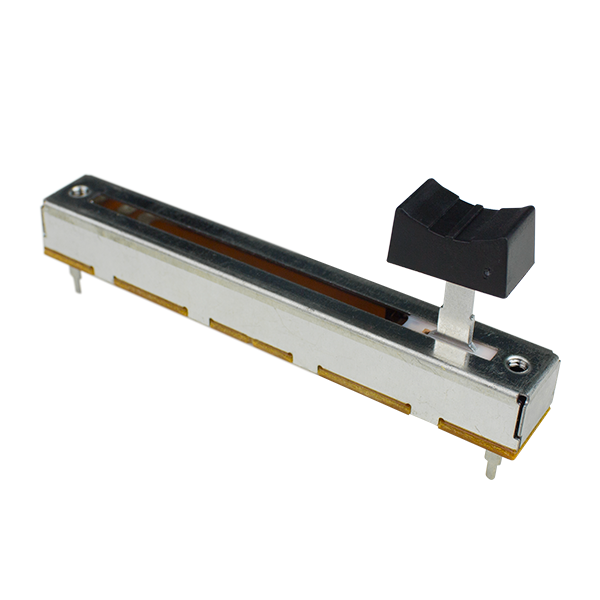
\includegraphics[width=0.5\textwidth]{figuras/fig61.png}
    \caption{botão \textit{slider} horizontal para frequência central \cite{robocore}}
    \label{fig61}
\end{figure}

A chave de duas posições será utilizada para selecionar entre dois efeitos distintos, gerando dois níveis de tensão: um nulo e outro de alimentação. Cada nível corresponderá a um efeito diferente. Um exemplo de botão para essa finalidade é mostrado na Figura \ref{fig62}.

Para ajustar a quantidade de efeitos desejada, será utilizado um botão semelhante ao \textit{slider}, com a mesma abordagem de controle e ajuste.

\begin{figure}[h]
    \centering
    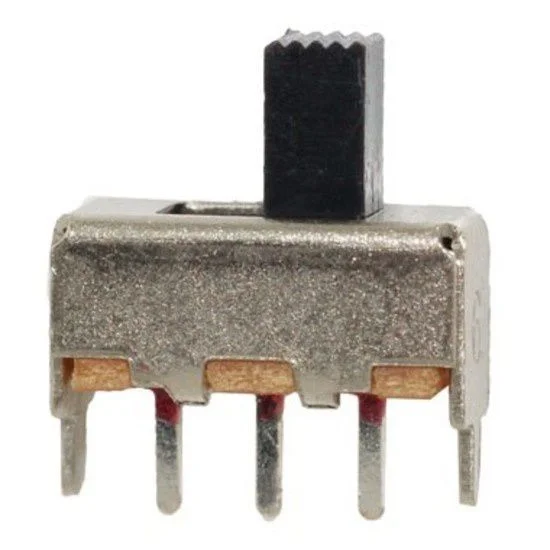
\includegraphics[width=0.3\textwidth]{figuras/fig62.png}
    \caption{botão de duas posições para seleção do efeito \cite{evea}}
    \label{fig62}
\end{figure}


\paragraph{Conversão AD}

A conversão analógica-digital será empregada em duas categorias de sinais: áudio e controle. Para cada categoria, diferentes níveis de quantização serão utilizados: um alto para garantir a definição das músicas convertidas e outro baixo para permitir a precisão necessária na identificação do efeito desejado (com dois níveis) ou da frequência central.

Para a conversão dos sinais analógicos de áudio, serão utilizados conversores de 16 \textit{bits}, como o mostrado na Figura \ref{fig63}.

\begin{figure}[h]
    \centering
    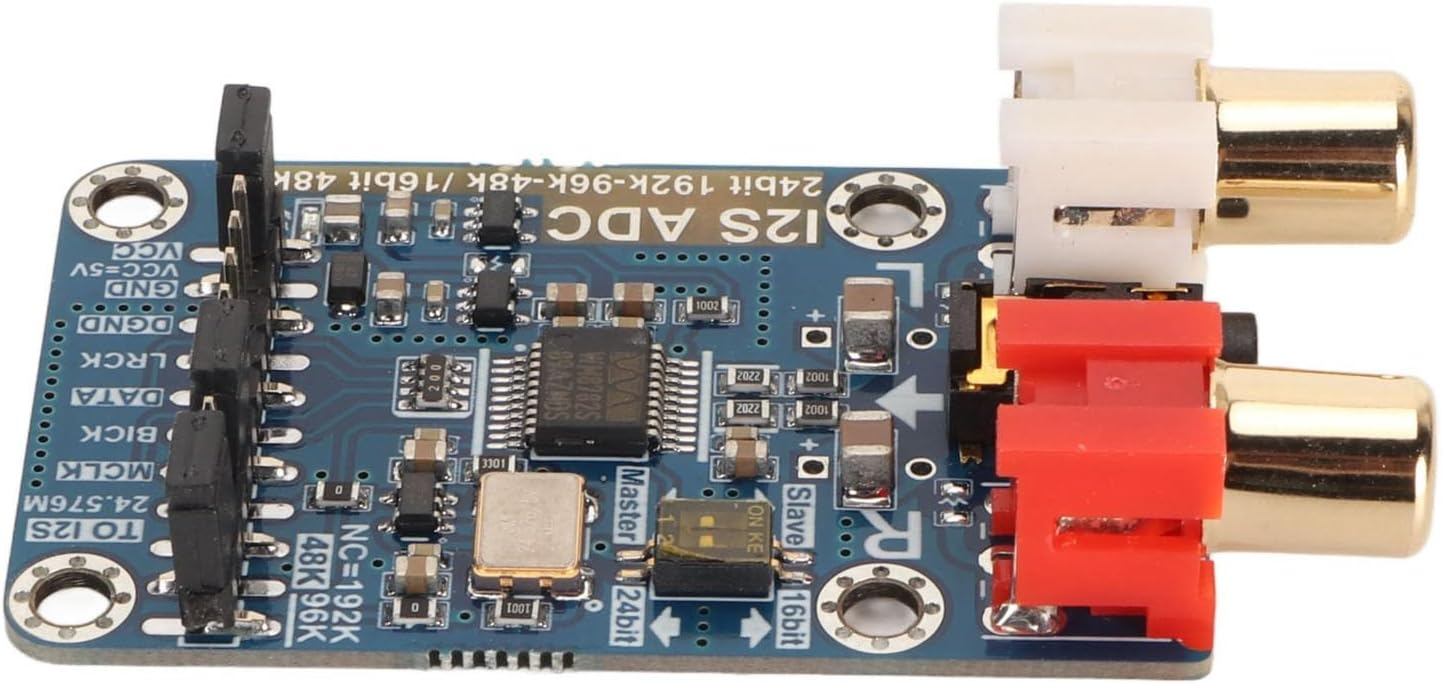
\includegraphics[width=0.5\textwidth]{figuras/fig63.jpg}
    \caption{conversor analógico-digital \cite{walmartRobotHuman}}
    \label{fig63}
\end{figure}

Para os sinais de controle, a conversão será realizada por um \textit{Arduino Uno}, que possui uma resolução de 10 \textit{bits}. O microcontrolador utilizado está representado na Figura \ref{fig64}.

\begin{figure}[h]
    \centering
    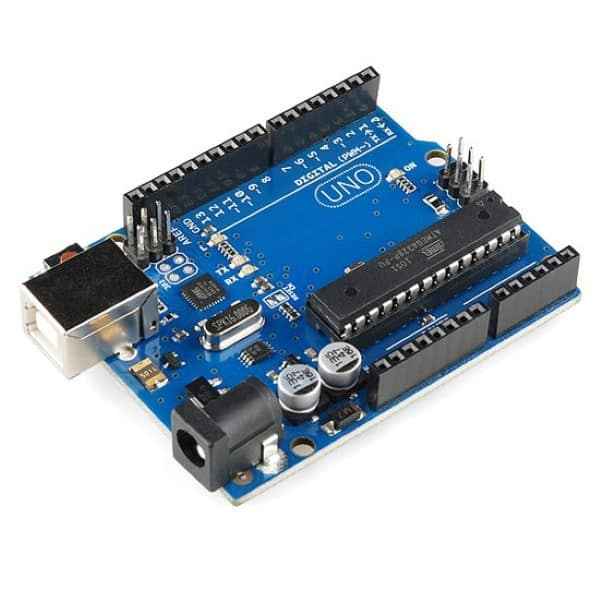
\includegraphics[width=0.5\textwidth]{figuras/fig64.jpeg}
    \caption{\textit{Arduino Uno} para conversão de sinais de controle \cite{vidadesilicioPlacaCabo}}
    \label{fig64}
\end{figure}

\paragraph{Protocolos de Comunicação}
Com conversores analógico-digital adequados, os sinais podem ser adquiridos e interpretados pela \textit{Raspberry Pi}. Existem várias maneiras de adquirir esses sinais analógicos a partir de um dispositivo, sendo uma das mais eficientes o uso de protocolos de comunicação serial, que permitem a transmissão e/ou recepção de sinais através de um canal de comunicação.

Para esta aplicação, recomenda-se o uso de diferentes canais de comunicação para sinais de áudio e sinais de controle. Os protocolos de comunicação devem ser compatíveis com os conversores utilizados.

Para a recepção de sinais de áudio, o \textit{mixer} utilizará o protocolo I2C, que é suportado pelos conversores selecionados. Já para a recepção dos sinais de controle, os protocolos disponíveis incluem UART (\textit{Asynchronous Receiver/Transmitter}), I2C (\textit{Inter-Integrated Circuit}) ou SPI (\textit{Serial Peripheral Interface}).

\paragraph{Unidades de Processamento}

A unidade de processamento é o dispositivo responsável pela realização do processamento dos sinais. Para essa tarefa, será utilizada uma \textit{Raspberry Pi}, que oferece um bom poder de processamento e flexibilidade em termos de linguagens de programação suportadas. A \textit{Raspberry Pi} é mostrada na Figura \ref{fig65}.

\begin{figure}[h]
    \centering
    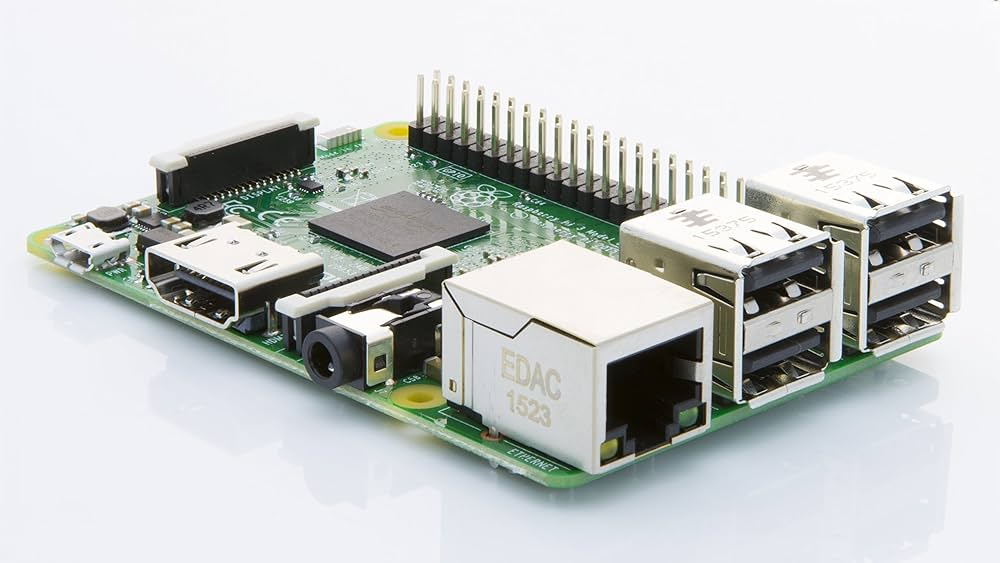
\includegraphics[width=0.5\textwidth]{figuras/fig65.jpg}
    \caption{\textit{Raspberry Pi} para processamento dos sinais \cite{adrenalineDisplaysLanar}}
    \label{fig65}
\end{figure}

\paragraph{Conversão DA}

A conversão digital-analógico é necessária para que o sinal final, após o processamento, possa ser reproduzido por sistemas de áudio que utilizam sinais analógicos. A \textit{Raspberry Pi} possui uma saída/entrada de áudio com conector de 3.5mm, conforme ilustrado na Figura \ref{fig20}.

\subsection{Implementação em Software}

Na \textit{Raspberry Pi}, após a conversão e aquisição dos sinais, é necessário realizar o processamento para obter o sinal final. Devido à sua eficiência no processamento, a linguagem C será utilizada para a implementação do sistema.

\subsection{Protótipo de Interface de Usuário}

A interface do usuário será projetada de forma semelhante a um \textit{mixer} atual, com dois botões \textit{sliders} horizontais e um botão de duas posições. Na parte traseira do dispositivo, estarão localizados os conectores \textit{RCA} e a entrada de alimentação.
